\section{Zielsetzung}
Das vorliegende Experiment dient dazu, gekoppelte Schwingkreise und die vorkommenden Phänomene näher zu untersuchen.
Hierzu werden, der Einfachheit sowie Genauigkeit halber, elektrische Schwingkreise genutzt.


\section{Theorie}
\subsection{Grundlagen des gekoppelten Schwingkreises}
\label{sec:Theorie}
Der Grundaufbau des gekoppelten Schwingkreises wird in Abbildung \ref{fig:schwingkreis} beschrieben.

\begin{figure}[H]
  \centering
  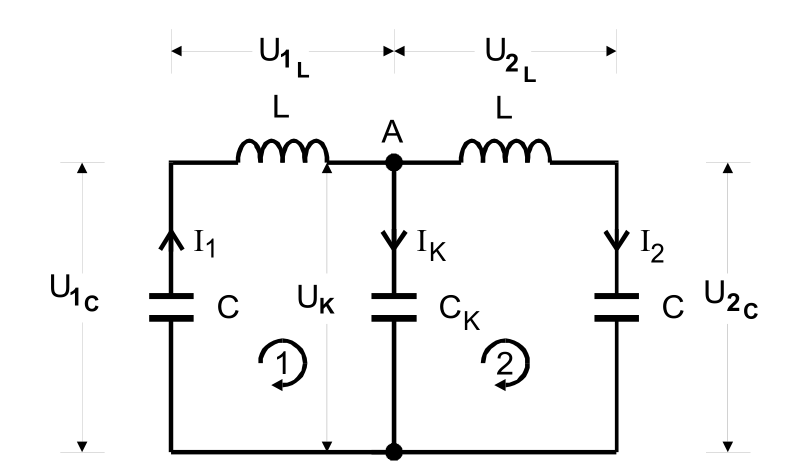
\includegraphics[height=6cm]{kreis.png}
  \caption{Schwingkreis. \cite{sample}}
  \label{fig:schwingkreis}
\end{figure}

Die Beschreibung der Ströme und Spannungen folgt dabei aus den Kirchhoffschen Regeln.
Die erste Kirchhoffsche Regel ist dabei die Knotenregel \eqref{eqn:knotenregel}.
Diese folgt direkt aus der Ladungserhaltung und besagt, dass in jedem Knotenpunkt einer Schaltung die Summe alle eingehenden und ausgehenden Ströme verschwinden muss:
\begin{equation}
  \sum_{k=1}^n I_k = 0.
  \label{eqn:knotenregel}
\end{equation}
%Beispielsweise gilt für Abbildung \ref{fig:knotenregel}
%\begin{equation}
%I_1 = I_2 + I_3
%\end{equation}
%\begin{figure}[H]
%  \centering
%  \begin{tikzpicture}
%    \draw[->] (0, 0) -- (1.8, 0) node[midway, above] {$I_1$};
%    \draw[->] (2, 0.1) -- (4, 1) node[midway, above] {$I_2$};
%    \draw[->] (2, 0) -- (4, 0) node[midway, below] {$I_3$};
%    %\draw[IPfeil=0em]([yshift=1.0em]0,0) -- node [above]{I$\mathsf{_R}$}([yshift=1.0em]0.5,0);
%  \end{tikzpicture}
%  \caption{Maschenregel.}
%  \label{fig:knotenregel}
%\end{figure}
Die zweite Kirchhoffsche Regel ist die Maschenregel \eqref{eqn:maschenregel}.
Sie folgt aus dem Induktionsgesetz im Vakuum
\begin{equation}
\oint \vec{E} \cdot \vec{\symup{d}s} = 0
\end{equation}
und besagt, dass in jeder geschlossenen Masche der Schaltung die Summe der Spannungen null ergeben muss:
\begin{equation}
  \sum_{i=1}^n U_i = 0.
  \label{eqn:maschenregel}
\end{equation}
%Beispielsweise gilt für Abbildung \ref{fig:maschenregel}
%\begin{equation}
%U_s = I \cdot R_3 + I \cdot R_2 + I \cdot R_1
%\end{equation}
%\begin{figure}[H]
%  \centering
%  \begin{tikzpicture}[circuit ee IEC, font=\sffamily\footnotesize]
%      \draw (0,0) to [resistor={info={$R_1$},info'={$\mathsf{_{}}$}}] (4,0);
%      \draw (4,0) to [resistor={info={$R_2$},info'={$\mathsf{_{}}$}}] (4,2);
%      \draw (4,2) to [resistor={info={$R_3$},info'={$\mathsf{_{}}$}}] (0,2);
%      \draw (0,2) to [battery={info'={$U_s$}}] (0,0);
%      %\node at ([xshift=-1em]battery.north) {+};
%
%      \draw[IPfeil=0em]([yshift=1.0em]1.7,2.1) -- node [above]{$I$}([yshift=1.0em]2.3,2.1);
%    \end{tikzpicture}
%    \caption{Maschenregel.}
%    \label{fig:maschenregel}
%\end{figure}

Um die an einem Kondensator sowie an einer Induktivität anliegenden Spannungen zu beschreiben, werden zudem die Beziehungen
\begin{equation}
  U_C = \frac{1}{C} \int^{} I \symup{d}t
\end{equation}
sowie
\begin{equation}
 U_L = L \frac{\symup{d}}{ \symup{d}t} I
\end{equation}
genutzt.
Es folgen somit jeweils für die beiden Maschen im Schwingkreis die Gleichungen
\begin{equation}
  \frac{1}{C} \int^{} I_{1} \symup{d}t + L \frac{\symup{d}}{ \symup{d}t} I_{1} +   \frac{1}{C_k} \int^{} (I_{1} - I_{2}) \symup{d}t =0
\end{equation}
beziehungsweise
\begin{equation}
  \frac{1}{C} \int^{} I_{2} \symup{d}t + L \frac{\symup{d}}{ \symup{d}t} I_{1} +   \frac{1}{C_k} \int^{} (I_{2} - I_{1}) \symup{d}t =0 .
\end{equation}
Durch erneutes Ableiten dieser Gleichungen erhält man das Differentialgleichungssystem der beiden Gleichungen
\begin{equation}
  \frac{\symup{d^2}}{ \symup{d}t^2} I_1 + \frac{1}{LC} I_1 + \frac{1}{L C_k} (I_1 - I_2) =0
\end{equation}
und
\begin{equation}
  \frac{\symup{d^2}}{ \symup{d}t^2} I_2 + \frac{1}{LC} I_2 + \frac{1}{L C_k} (I_2 - I_1) =0.
\end{equation}
Dieses System lässt sich durch Entkopplung in die Stromsumme $I_1 + I_2$ sowie die Stromdifferenz $I_1 - I_2$ lösen, wobei sich als Lösungen
\begin{equation}
  \label{eqn:strom1}
  I_1(t) = \frac{1}{2} (I_{1,0} + I_{2,0}) \cos{\omega_1 t} + \frac{1}{2} (I_{1,0} - I_{2,0}) \cos{\omega_2 t}
\end{equation}
sowie
\begin{equation}
  \label{eqn:strom2}
  I_2(t) = \frac{1}{2} (I_{1,0} + I_{2,0}) \cos{\omega_1 t} - \frac{1}{2} (I_{1,0} - I_{2,0}) \cos{\omega_2 t}
\end{equation}
ergeben, wobei $I_{1,0}$ und $I_{2,0}$ die jeweiligen Anfangsbedingungen für $I_1$ und $I_2$ sind.
Die sich ergebenden Fundamentalfrequenzen $\omega_1$ und $\omega_2$ betragen
\begin{equation}
  \omega_1 = \frac{1}{\sqrt{LC}}
  \label{eqn:omega1}
\end{equation}
und
\begin{equation}
  \omega_2 = \sqrt{\frac{ \frac{1}{C} + \frac{2}{C_k} }{ L }}.
  \label{eqn:omega2}
\end{equation}
Für die beiden Anfangsbedingungen $I_{1,0} = I_{2,0}$ beziehungsweise $I_{1,0} = -I_{2,0}$ ergeben sich die beiden Fundamentalschwingungen des Systems.
Diese zeichnen sich dadurch aus, dass im ersten Fall das System mit der Frequenz $\omega_1$ sowie einer Phasenverschiebung von $\phi = 0$, im zweiten Fall mit einer Frequenz von $\omega_2$ sowie einer Phasenverschiebung von $\phi = \frac{\pi}{2}$ oszilliert. \\
Werden die Anfangsbedingungen so gewählt, dass ein Startstrom auf $I=0$ gesetzt wird, so ergeben sich aus den allgemeinen Lösungen \eqref{eqn:strom1} und \eqref{eqn:strom2} nach Anwendung von Additionstheoremen
\begin{equation}
  I_1(t) = I_{1,0} \cos{\frac{1}{2} (\omega_1 + \omega_2) t} \cos{\frac{1}{2} (\omega_1 - \omega_2) t}
\end{equation}
beziehungsweise
\begin{equation}
  I_2(t) = I_{1,0} \sin{\frac{1}{2} (\omega_1 + \omega_2) t} \sin{\frac{1}{2} (\omega_1 - \omega_2) t}.
\end{equation}
Es handelt sich hierbei um Schwebungen, bei denen die Stromamplituden mit einer Schwebungsfrequenz von
\begin{align}
  \omega_s = \frac{\omega_2 - \omega_1}{2}
  \label{eqn:omega_s}
\end{align}
sowie einer Überlagerungsfrequenz von
\begin{align}
  \omega_r = \frac{\omega_1 + \omega_2}{2} \approx \omega_1
  \label{eqn:omega_r}
\end{align}
oszillieren.
Der Phasenunterschied beträgt nun $\phi = \frac{\pi}{2}$, die Gesamtenergie oszilliert periodisch zwischen den beiden Schwingkreisen.
Damit dieser Zustand auch in der Praxis erreicht werden kann, ist es nötig, in beiden Maschen die Werte für $L$ und $C$ identisch zu wählen, so dass die Resonanzfrequenz in beiden Schwingkreisen identisch wird.
Nur so kann die Energie möglichst verlustfrei oszillieren.
\subsection{Gekoppelter Schwingkreis mit erzwungener Spannung}
Im Folgenden wird der in Abbildung \ref{fig:sinus_schwingkreis} dargestellte Schwingkreis betrachtet.
\begin{figure}[H]
  \centering
  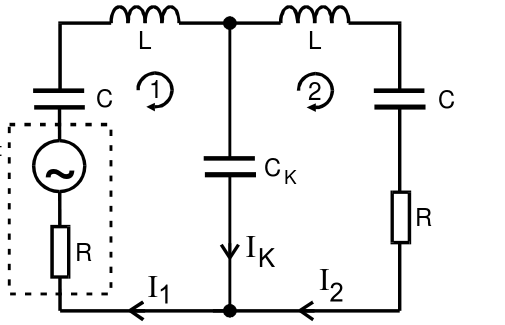
\includegraphics[height=6cm]{sinus_theorie.png}
  \caption{Schwingkreis mit Sinusspannung. \cite{sample}}
  \label{fig:sinus_schwingkreis}
\end{figure}
Anders als beim bisher betrachteten Aufbau wird der Schwingkreis nun mit einer Sinusspannung von
\begin{equation}
U(t) = U_0 \exp(i \omega t)
\end{equation}
getrieben.
Aus der Maschenregel \eqref{eqn:maschenregel} folgt für die beiden Maschen der Schaltung
\begin{equation}
  I_1 R + I_1 Z_C + I_1 Z_L + I_k Z_{C,k} = U_0
\end{equation}
und
\begin{equation}
  I_2 R + I_2 Z_C + I_2 Z_L - I_k Z_{C,k} = 0.
\end{equation}
Nach Anwendung der Knotenregel \eqref{eqn:knotenregel} sowie der Impedanzen
\begin{equation}
  Z_C = \frac{-i}{\omega C},
\end{equation}
\begin{equation}
  Z_L = i \omega L
\end{equation}
erhält man für den Betrag von $I_2$
\begin{equation}
 \lvert I_2 \rvert = \frac{U_0}{ 4 \omega^2 C_k^2 R^2 Z(\omega)^2 + \Bigl( \frac{1}{\omega C_k} - \omega C_k Z(\omega)^2 + \omega R^2 C_k \Bigr)^2 }
   \label{eqn:idoof}
\end{equation}
mit
\begin{equation}
  Z(\omega) = \omega L - \frac{1}{\omega} \Bigl( \frac{1}{C} + \frac{1}{C_k} \Bigr).
\end{equation}
Bestimmt man das Maximum von $I_2$ in Abhängigkeit von $\omega$, so zeigt sich, dass der Strom für die beiden Fundamentalfrequenzen $\omega_1$ \eqref{eqn:omega1} sowie $\omega_2$ \eqref{eqn:omega2} maximiert wird.
Das Strommaximum beträgt dabei für beide Frequenzen genähert
\begin{equation}
  I_{2,max} \approx \frac{U_0}{2R}.
\end{equation}
\cite{sample}
